% arara: xelatex: { shell: yes, synctex: yes }
% arara: biber if (missing("bbl") || changed("bib"))
% arara: xelatex if (missing("bbl") || changed("bbl"))
% arara: xelatex if (found("log", "Rerun to get cross-references right."))
\RequirePackage[l2tabu, orthodox]{nag}
\documentclass[english,purist]{ist-report}

% ================ BEGIN PREAMBLE ================

\usepackage{siunitx}
\sisetup{
	round-mode		= places,
	round-precision	= 2,
}

\usepackage[sfdefault]{FiraSans} %% option 'sfdefault' activates Fira Sans as the default text font
\renewcommand*\oldstylenums[1]{{\firaoldstyle #1}}
\usepackage{FiraMono}
\usepackage{newtxsf}

\usepackage{amssymb}
\usepackage{textcomp}
\usepackage{gensymb}
\usepackage{cancel}

\usepackage{biblatex}
\addbibresource{main.bib}

\usepackage{fvextra}
\usepackage{csquotes}
\usepackage{booktabs}
\usepackage{enumitem}
\setlist{noitemsep}

\graphicspath{{graphics/}}
\usepackage{caption}
\usepackage{subcaption}
\captionsetup{width = 0.9\textwidth}

\usepackage{tikz}
\usepackage{pgfplots}
\usetikzlibrary{arrows.meta,positioning,patterns}
\pgfplotsset{
	compat=1.15,
	table/search path = {data},
	/pgf/number format/use comma,
}

\usepackage{todonotes}

\author{Pedro Afonso \\ 66277 \and João Manito \\ 73096 \and Daniel de Schiffart \\ 81479}
\title{Electronic Warfare Aeronautical Systems}
\subtitle{Research Report}
\date{December 2018}
\subject{Integrated Avionics Systems}
\course{Integrated Masters in Aerospace Engineering}

\newrobustcmd*{\jamming}{\textit{jamming}}

% ================= END PREAMBLE =================

\begin{document}

\makecover{}

\begin{abstract}
	In this research report we will present a general discussion on the topic of electric and electronic aeronautical systems and their presence within the context of war and warfare, beginning with an historical overview of the presence of these systems in aeronautics, their growth and expansion, the detection and exploitation of their vulnerabilities and subsequent and ongoing battle between exploitation and protection of these systems. Following it will be a presentation of the most notable weapons and systems within this topic, both historical and modern, which will culminate in a discussion on the future of electronic aeronautical systems and how relevant their overall protection  can be to modern safety in the aeronautical and aerospace industry.
\end{abstract}

{\hypersetup{linkcolor={black}} \tableofcontents}

\pagebreak

\section{Introduction}\label{sec:introduction}
Electronic Warfare is defined as a set of measures and actions
performed by the conflicting sides to detect and electronically attack enemy electronic systems for the control of forces and weapons, including high precision weapons, as well as to electronically defend one's own electronic systems and other targets from technical intelligence (electronic intelligence, ELINT), jamming and non deliberate interference.  
Electronic attack can be achieved by:
\begin{itemize}
    \item Jamming (active, passive, false targets);
    \item Reduction of radar and thermal detectability;
    \item Changing the electrical properties of the environment (conditions
for the propagation of electromagnetic waves). 
\end{itemize}

Typically, EW methods of operation can be either offensive or
defensive in nature. When we speak of offensive operations, first and
foremost we have in mind operations conducted using jamming or employing weapon systems that automatically home in on radiation sources. Both of these offensive operation methods are used not only to attack (or destroy) electronic systems for the control of forces and weapons, but also to defend one's own electronic systems against ELINT and jamming.

In the first instance, the jamming targets are the receivers of radar,
communications, and radio navigation systems. In the second case, the
jamming targets are ELINT receivers that form a part of active jamming and ELINT stations, as well as of reconnaissance and strike systems.

Typical defensive EW operations involve protecting the respective
systems from jamming and ELINT by increasing their equivalent specific
energy potential, modifying their time, frequency, space and other characteristics, or by making them more secure (masking, deception).

As a rule, the most effective solution to the problem of protecting
against jamming is achieved by combining both purely defensive and
offensive operations. More precisely, this is achieved by destroying the jammer or by electronically jamming ELINT systems and active jammers. Thus, it may be said that jamming and ELINT, taken together, by and large comprise the basis of EW. 

When viewing radar and other electronic devices as targets of E\textbackslash x!
(jamming), we should keep in mind that jamming signals directly affect radio receivers. A priori, as a rule, the jammer or other electronic attack system does not have full information about the target of the attack. In order to eliminate the element of chance for the victim receiver, it should be attempted to orient oneself by assuming that the victim system uses optimum or quasi-optimum processing methods for the signals received and within a certain standard (conditional) electronic environment. Depending on how the radar or other electronic device operates, differing variants of processing optimization may occur, thus resulting in various mathematical models.

\part{History}

The nature of warfare and the history of the development of any warfare technology is to develop and implement superior tools of war and deny the opponent the same privilege. With that in mind, the story of the development of electronic warfare can best be described by Newton's third law, which states
\begin{quote}\itshape
    For every action, there is an equal and opposite reaction.
\end{quote}
The growth of the technologies of war can not only be described by the advances made by either side of a war, but also by the progress made by the opposing sides in denying said advance. Such is the story of the dichotomy of electronic warfare, both in the offensive (attacking) and defensive (protecting) fronts of development.

\section{Early Beginnings} 

\subsection{First known instance}

The story of electronic warfare can have different begins based on what the actual definition of the term entails and is considered to be, regarding both halves of the term. The \emph{electronic} part, where a definition of what constitutes a useful application of electricity and electronic components, and the \emph{warfare} side of the term, where ambiguity can be found on what could be actually considered as deliberate attacking action and protection thereof within the electronic realm.

Ambiguities aside, a good starting point can be traced all the way back to the time of the civil war of the United States of America, where the early developments of the telegraph by Samuel Morse and their uses in the war gave their users (in this case, the Union forces) clear advantage in long distance communication\footnotemark. To counteract this advantage, the Confederate forces rerouted telegraph wires, forged fake communications, or straight up cut the communication channels. This can be traced all the way back to the start of the civil war in 1861 as the first recorded example of signal jamming, and therefore, the \textbf{first known instance of electronic warfare}.
\footnotetext{As mentioned in \textcite{alican2006}. Most of this section was written using references \textcite{armytechnology} and \textcite{price1977} as well as the aforementioned reference.}

\subsection{Beginning of \textit{modern} electronic warfare}

With the emergence of radio technology, demonstrated by Heinrich Hertz in 1888, the transmission of Morse code became less restricted to physically mounted transmission lines and could be used for long-range communications with much more facility than ever before. Quickly these systems became commonplace, first with a focus on civilian use and not much later for military use.

With these developments, the interest in disrupting these \textit{wireless} communications became bigger. Approaching the more modern definition of electronic warfare, the objective was set at intercepting or blocking these communications entirely. The first recorded instance of radio \jamming{}, as the procedure quickly came to be known as, occurred in 1901 in the United States of America, in a civilian yacht race.
\begin{quote}\itshape
    The first recorded instance of deliberate radio jamming took place in
September 1901, in the U.S. Interestingly, it was aimed at securing
commercial gain rather than military advantage. As now, there was
considerable public interest in the America’s Cup yacht races, and the
newspaper first to reach the stands carrying each result stood to reap a
large profit. In that year, Marconi obtained a contract from Associated
Press [...] Another company, [...] Wireless Telegraph Company of America,
secured a contract [...] A third company, the American Wireless Telephone
and Telegraph Co., [...] failed to get a sponsor but decided to exploit the
situation (and)[...] used a transmitter more powerful than its competitors,
and one of its engineers, John Pickard, worked out a method which
allowed him to jam signals from the other companies while at the same
time reporting on the progress of the race from his boat [...] thus only AWT
\& T was able to pass accurate reports on the races. \cite{alican2006}
\end{quote}
This event effectively marked \textbf{the first occasion of offensive \jamming{}} and therefore the \textbf{first occurence of modern electronic warfare}. Although the event didn't accumulate much military attention, radio \jamming{} was becoming widely implemented and experimented with in military exercises, first by the British Navy in 1902 and by the U.S.\ Navy in 1903. This set precedents for western countries and their respective military forces to counteract the ever-increasing use of radio.

In the eastern warfronts, the appearance of \jamming{} came by the Russians in the 1904-1905 Russo-Japanese war, which marked the first known war in which both sides used radio communications.

\subsection{Growth and expansion of radio}

In a period of relative peace and quick scientific progress, this new-found technology was developing rapidly. The beginning of the 20th century saw radio technology improve its transmission ranges, and more channels were being introduced by the narrowing of channel bandwidths. Not only that, but the transmitter and receiver technologies were being continually improved, and as a result, interference was lowering and communications became clearer.

Portability of radio systems was improving as well, which made the pairing with the emergent aeronautical field an obvious choice. Soon enough, aeroplanes were being fitted with radio communications.

\section{World War 1}

The spark of the first major World War, \textit{the war to end all wars}, made the first real testing scenario for a lot of emerging warfare technology in all fields, from weapons to transportation to information to communication, and at the forefront of this last topic lied the radio.

By this point, most countries involved in the war had implemented and exercised with some form of signal \jamming{}, with the remaining countries quickly catching up. But the functionality and importance of this technology and of radio communications wasn't fully understood by their users, and most mid-battle signal \jamming{} occurred between friendly forces, when too many radio communications being attempted within a small space.

Towards the end of World War 1, the use of radio communications was so widespread that its presence could be exploited by either side of the war. A notable example was the detection of German U-boats in the Mediterranean, which started as a major threat to Allied forces in the battle for the sea, but whose detection and persecution became trivialised by the implementation of primitive direction finders that worked based on the communications performed by these underwater vessels.

\section{War Aftermath and Further Developments}\label{sec:betweenwars}

World War 1 was, up to that point, the biggest stage for military use of radio and the then-emerging field of electronic equipment and technology in the military, and the potential was present. With the desire of a lasting peace, the countries involved in the war agreed to organise and prevent similar events from happening again, but the mistrust created meant that while peace looked possible, all the parties involved were preparing themselves should the need arise again.

With the aforementioned potential, this meant that research was going to develop quickly, specially without the pressure of short-term war. In the period after the war, radio-transmitting equipment had its weight and size reduced, its reliability and performance improved, and its implementation for various uses widespread, which raised overall population education with the technology. This meant that communication between land, sea, and air was continually improving.

\subsection{RADAR}

A major breakthrough happened in this period with the appearance of \textbf{RADAR}\footnote{\textbf{RA}dio \textbf{D}etection \textbf{A}nd \textbf{R}anging.} in the early 1930s, which came as a consequence of the developments listed previously. This technology allowed for the detection of incoming traffic and enemy forces from very long distances with a similar technology as radio, and soon enough radar would be implemented in military forces worldwide. By the end of the 1930s, radar technology would develop from detecting aircraft at 30 kilometres to detecting them at 160 kilometres, with the major obstacle becoming the radius of the Earth.

This quickly prompted the emergence of countering technology. With radars being so widespread, a way to approach enemy bases undetected would be a major warfare advantage, so development gained expedience in methods to avoid detection or disabling radars from afar by \jamming{} them in much the same way as it is done with radio communications. Around this time, the first tests with this purpose in mind were done in London using continuous wave transmitters directed at the radar.

Quickly enough, radar \jamming{} became commonplace.

\section{World War 2}

If World War 1 was a showcase of the potential of electronics in the battlefield, World War 2 would meet a much more mature field of the exploitation of the electromagnetic spectrum in tools of war. With the development highlighted in section \ref{sec:betweenwars}, radio communication and navigation and radar would give significant advantages to their respective users. A key in disrupting communication and flow of intelligence in either side would be the effective development and use of methods of \jamming{} and interception, effective tools of electronic warfare.

\subsection{\textit{Battle Of The Beams}}

A notable example of electronic warfare in World War 2 occurred in the beginning of the war, a period in which the Axis forces (namely German forces) increased the use of radar and used the technology for \textit{blind} bombing in the United Kingdom \cite{wizardwar}.

Using diverse radio navigation systems, the Germans had accurate bombing ranges of up to 200 nautical miles from their fronts while completely in visual nighttime darkness.
\begin{figure}[ht]
    \centering
    \missingfigure[figwidth = \textwidth]{Add reference maps for the German radars}
    \caption{Map of the German radars used for the night bombings of the \textit{Battle Of The Beams.}}
    \label{fig:botb_map}
\end{figure}

The British forces were forced to implement counter-measures to the German radars by \jamming{} their signals accordingly. However, the technology used was unknown by the British, so they were forced to adapt depending on what intelligence could be gathered.

The first used radar technology, \textit{Knickebein}, was countered by mimicking the signals sent by German forces to the pilots to force them to drop bombs in safe areas and land wherever the signals guided them to do. Some German pilots even end up landing in British bases believing they were in Germany, as visual darkness prevented them from distinguishing one from the other.

The Germans countered this by implementing different technologies, named \textit{X-Gerät} and later \textit{Y-Gerät}, unknown to the British, which meant new counter-measures had to be found. These technologies were effectively shut down when the Allied forces found intelligence within crashed bombers that allowed them to jam the correct German-used frequencies.

The titled \textit{Battle Of The Beams} period ended when the German air force \textit{Luftwaffe} attention diverted to the Soviet Union front. But this period highlighted the \textbf{measure-counter-measure nature of electronic warfare} in the World War 2, an element of electronic warfare which persists to this day.

\subsection{Further War Development}

The British had learned lessons within the field and moved on from defence to offence, by beginning to implement aircraft-detection \textit{jammers}, namely the airborne \textit{Mandrel} \cite{alican2006}. The \textit{Mandrel} swamped the return echo of the enemy radars, distoring reception sizes and ranges and difficuling accurate detection.

Later on, both sides of the war would see widespread use of \textit{chaff}, called \textit{window} by the British and \textit{düppel} by the Germans, which consisted of materials dispersed in the air to create false radar positives to conceal real threats.
\begin{figure}[ht]
    \centering
    \missingfigure[figwidth = \textwidth]{Add image of radar chaff}
    \caption{\textit{Chaff}, material used to create false radar echoes.}
    \label{fig:chaff}
\end{figure}

Massive use of passive \textit{jammers} by English bombers started on June 24, 1943 during the nighttime bombing raid on Hamburg and continued systematically in subsequent raids. The \jamming{} targets were \textit{Wiirzburg} gunlaying radar stations, which had an emitted signal wavelength of about \SI{50}{\centi\meter}. In this case, the passive jamming consisted of manually launched tinfoil strips (dipoles) of the order of \SI{25}{\centi\meter} in length (i.e., equal to approximately half the radar wavelength). As a result of this jamming, bomber losses decreased by about half for several months. This use of \jamming{} was preceded by lengthy reconnaissance of the \jamming{} targets. The decision to employ \jamming{} was made after losses reached the maximum permissible level.

To a large extent, this \jamming{} was so highly effective due to the
wavelength selected for the \textit{Wiirzburg} radar. The absence in it of circuits to protect against passive \jamming{}, which appeared only at the end of the war; and the absence of the possibility to change wavelength. In October 1943, U.S. bombers began employing active jamming against \textit{Wiirzburg} radar using carpet-type \textit{jammers}, which turned out to be highly effective because it was not possible to alter the carrier frequency.

In the pacific front, \jamming{} saw widespread use, but little to no development.

\section{Post-War Development and Other Trials}

The biggest stage for electronic warfare had just passed and with it came several advancements in relevant warfare technology, in which numerous resources and man-hours were invested due to the urgency and necessity for these technologies in the middle of all-out war between many developed countries. The arrival of peace allowed for more experimentation with the advancements of wartime, but warfare trials for any developed tools would not arrive in the same scale as the one that just passed. Still, the years that followed World War 2 would still see scattered warfare with numerous chances for implementation of new technology.

With the standardisation of electronic warfare, other aspects of each armed forces were starting to take notes. Air tactics now had to consider heavily the presence of enemy radars and develop manoeuvres and procedures to avoid detection, and the emergence of \textbf{stealth} technology meant a whole new field of engineering which would see a lot of investment. This period would also see the first appointment of Electronic Warfare Officers.

It is possible to distinguish approximately four basic phases of significant change in the structure and algorithms of both radar and electronic warfare systems. The period of the 1950s corresponds to the development of non-coherent radar with rapid alteration of the carrier frequency and anti-\jamming{} devices built using pulse-to-pulse cancellation. In \textit{jammers}, electronic frequency alteration was introduced. Special devices for the launching of chaff were developed.

This period also saw the invention of the first functional surface-to-air missile system, which saw the deployment of radar-guided missiles controlled from the ground to meet and annihilate airborne targets. This soon prompted the beginning of development of counter-\jamming{} of these systems.

\section{Two Global Superpowers}

The Cold War that covered most of the second half of the 20th century was heavily reliant on intelligence and the protection thereof, as both sides of the war, the U.S.A. and the ever-growing U.S.S.R., wanted to develop as many tools of war as possible while hiding their information from the opponent. Thus gathering opposing force intelligence was, at the time, of major importance, but was also a major risk, as both parties were not officially at war with each other, and either side being caught stealing technology from the other could risk starting war, or \textit{setting off the keg}, as was commonly referred.

This meant that electronic warfare came to the forefront of intelligence gathering missions. Aircraft were being developed with more complex and advanced electronic warfare devices on-board, such as \textit{jammers}, radio, and computers. These aircraft were being steadily employed by the United States on Electronic Intelligence missions, now commonly referred to as ELINT missions.

At the time, the \textit{Lockheed U-2} was at the forefront of these developments. The aircraft was often used in these ELINT missions for gathering visuals of Soviet military and industrial installations and intelligence on Soviet radars and signals with the technology it carried on-board. With the widespread use of radar by both parties of the war, the aircraft was designed to gather a number of data from the enemy, including (but not limited to):
\begin{itemize}
    \item The rate of scanning of a radar beam, including direction and speed;
    \item Time width of radar pulses;
    \item Rate of radar pulses;
    \item Frequency of opponent emitters;
    \item Signals and emitter locations.
\end{itemize}
\begin{figure}[ht]
    \centering
    \missingfigure[figwidth = \textwidth]{Add image of the Lockheed U-2}
    \caption{The \textit{Lockheed U-2} aircraft, used by the United States of America for ELINT missions during the Cold War.}
    \label{fig:u-2}
\end{figure}

While remaining on \textit{friendly} terms with the Soviet Union, the United States performed several reconnaissance missions with this and several similar aircraft, until some were shot down by advancing anti-aircraft and anti-\textit{jamming} technology.

\section{The Vietnam War}

The late 50s and early 60s saw the United States joining the war in Vietnam. Fighting a war on foreign soil meant several problems for the joining forces, as they were entering the enemy's battlefield and would have to face the enemy's setup as opposed to preparing their own ground. Early in the war, the invading forces suffered numerous airborne casualties due to Vietnamese radars, surface-to-air missile systems and anti-aircraft units installed on their grounds, which could detect and intercept invading aircraft.

This saw the development of counter-measures to fight this type of tracking and detection, and new models of codenamed \textit{Wild Weasel} aircraft were shipping out equipped with Radar Homing and Warning systems, developed to shut down the aforementioned threats. These aircraft carried numbers of radar-seeking missiles, which would hone in on radar signals emitted by enemy forces to destroy them and provide cover for more ground-oriented bombers and other aircraft.
\begin{figure}[ht]
    \centering
    \missingfigure[figwidth = \textwidth]{Add image of a Wild Weasel}
    \caption{A \textit{Wild Weasel} aircraft, equipped with radar-seeking missiles and anti-SAM equipment.}
    \label{fig:wildweasel}
\end{figure}

This greatly facilitated the invasion and made the attack of heavily fortified areas possible without heavy casualties using a coordination of ground, sea, and air forces, but also reconnaissance and intelligence, as the anti-aircraft weaponry relied greatly on radar detection to remove airborne threats.

The Vietnam War very much highlighted the importance of correct knowledge and use of electronic warfare in the modern war landscape and its position as a key factor in the outcome of modern warfare.

\section{The First Gulf War -- Operation Storm and The Beginning of The Modern Age}

The first Gulf War at the beginning of the 1990s once again put the current status of electronic warfare and its importance to the test. Both sides and their arsenal were put to the test, and as proven time and time again, intelligence would play a major role in the final outcome.
\begin{figure}[ht]
    \centering
    \missingfigure[figwidth = \textwidth]{Add something relevant to the first gulf war}
    \caption{Something about the gulf war}
    \label{fig:gulfwar}
\end{figure}

The Iraqi military were setting up with massive amounts of anti-aircraft artillery and surface-to-air missile systems to contain the invasion of the coalition forces, and an imposing airborne arsenal comprised of a mix of old and new Soviet-developed aircraft.

Unlike previous war, despite the Iraqi communication, transportation, military and power infrastructure being well-run and providing their forces with the necessary power for battle, the coalition forces aimed for disabling their command and control system to turn the outcome of the airborne warfare in their favour.

This meant that the coalition would favour targets such as command posts, communication systems, anti-aircraft radars and electrical generation networks to debilitate the electronic warfare capabilities of the Iraqi forces.

A combination of radar decoys, \jamming{} aircraft and land-attack missiles were used to swiftly destroy air command and communications centres. Following these eliminations, technology developed from the radar-seeking missiles used in the Vietnam War was used to eliminate the Iraqi's radar-powered anti-aircraft capabilities. Decoys simulating larger aircraft were escorted by bombers to disperse Iraqi attention and distract them from the real targets, while providing cover for those bombers to infiltrate and reach advantageous positions for attack.

A host of targets in Iraq were also destroyed by stealth aircraft, which possess a very low radar signature and could fly in surveyed areas relatively undetected as long as it remained out of visual and audible detection. This meant that the overall airborne casualty count remained very low for the dimension of the battles fought.

Combined with a host of other technology unavailable to the Iraqi forces meant that the war quickly and swiftly swung in favour of the coalition forces. The first Gulf War marked the turning point of modern warfare, with electronic warfare securing its central position as deciding factor in the outcome of modern warfare.

\part{Electronic Attack}

\section{Introduction}

Electronic attack can be implemented by jamming, changing the electrical and magnetic characteristics of the environment, or by reducing the radar and thermal detectability of aircraft.
At the present time, the basic means of electronic attack in the radio
frequency band is the use of various jamming signals that directly affect electronic systems. These signals are deliberate electromagnetic emissions with the appropriate amplitude, frequency, phase, polarization, space and time characteristics. Practically speaking, jamming signals are·produced by jammers (electronic attack systems). 

In a given electronic environment, jammers are used in particular ways
depending on the specifics of the targets being jammed and the capabilities of the jammers. 

In the general case, electronic attack systems comprise an information
support and control system, a subsystem for producing jamming signals,
high-frequency amplifiers and generators with modulators, and antenna
devices. \textit{ELINT} systems, knowledge bases and computer data that enter into the \textit{EW} complex serve as the basis for the information support and control system. The \textit{ELINT} subsystem seeks out, receives and processes radio signals from jamming targets. By comparing signals coming in from \textit{ELINT} and a priori information contained in the knowledge base and computer data: 

\begin{itemize}
    \item The electronic environment is evaluated; 
    \item The jamming target is determined, as well as the type and
parameters of the jamming signal needed; 
    \item A means of attacking the jamming target is selected and executed. 
\end{itemize}

Jamming methods are determined by the characteristics of the jamming
targets and the abilities of jammers to cause information damage to the victim, given specific conditions of the operational and tactical environment. 

Information damage means the quantity of information that the attacked side loses during a specific time interval as a result of the effect of jamming or other \textit{EW} measures. 

Thus, jamming signals, as well as systems and techniques of jamming,
can be considered to be the basic elements of electronic attack.

Three types of jamming signals have been defined to date: destructive,
masking and deception. They also occur in combinations. As a rule, masking and deception jamming signals are additive. 

The basic targets for jamming using airplane and helicopter based jamming systems are \textit{AAD - Army Air Defense -} radar systems of various types (for control of \textit{AAD} forces and weapons etc...).
Besides these jammers, passive jamming is widely used, as well as optoelectronic jamming systems.

The determining element in a modern airborne jamming system is
automatic active jammers with an information support system permitting the control both of active and passive jamming systems and optoelectronic jamming systems in the dynamics of \textit{EW}.

A block diagram for an automatic jammer is given by the figure \ref{jam1}, which is the logical result of the analysis of a smoothed radar environment, occurring at the current time in the dynamics of \textit{EEW}. The structure of a jammer permits the
formation of jamming signals both for the jamming of radar systems for
control of \textit{AAD}forces and weapons. The information support system of the jammer and the jamming system as a whole are represented as an \textit{ELINT} station, with its processor, knowledge and databases, a receiver, and the processor of the jammer itself. Besides this, the information support system also contains onboard information systems: the central onboard computer with its knowledge- and databases, the onboard radar system, the onboard optoelectronic intelligence system, the navigation and data interchange (radio communications) systems, and, possibly, an automated control system for EW systems. 

A stream of signals from radar stations, which are the operations targets, arrive at the receiving antennas of the \textit{ELINT} devices and jammers. 

As a rule, while transmitting, \textit{ELINT} receivers are not able to detect signals from a radar irradiating the aircraft in the corresponding frequency band. 

After the radar signal has been detected, an analysis of the electronic environment is conducted and the operations target identified. Then, a jamming signal is generated. Depending on its type, either direct radiofrequency (RF) jamming (direct noise interference) is generated or jamming modulation of RF radiation is performed. Jamming signals are emitted in the appropriate direction by the jammer transmitter antennas. 



\begin{figure}[ht]
\centering
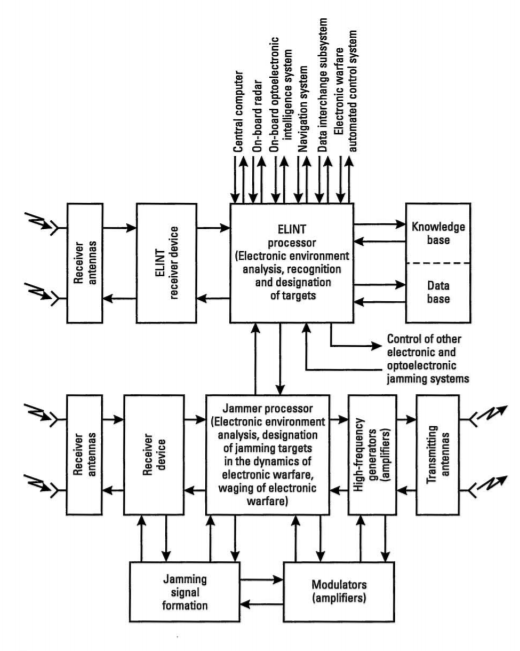
\includegraphics[width=70mm]{jam1.png}
\caption{Block diagram for an automatic jammer}
\label{jam1}
\end{figure} 

We can include methods of concealing airplanes (helicopters) and other targets from stationary areas, figure \ref{jam2}, using jamming; methods of screening helicopter or airplanes in battle formation, figure \ref{jam3}, using jamming; the mutual screening of airplanes
using electronic jamming systems; the self-screening of airplanes (helicopters) using electronic jamming systems; and the combination of electronic jamming with the destruction of electronic targets using firepower. 

\begin{figure}[ht]
\centering
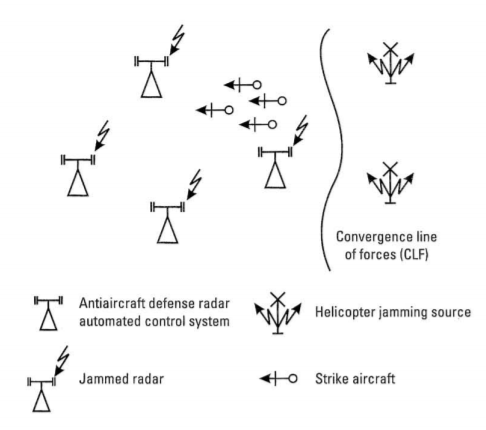
\includegraphics[width=70mm]{jam2.png}
\caption{Methods of concealing airplanes (helicopters) and other targets from fixed areas using jamming.}
\label{jam2}
\end{figure} 

\begin{figure}[ht]
\centering
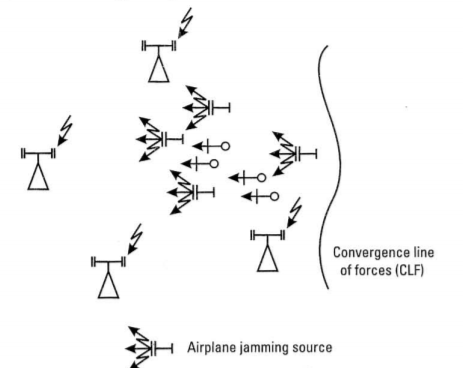
\includegraphics[width=70mm]{jam3.png}
\caption{Methods of screening airplanes in battle formation using jamming.}
\label{jam3}
\end{figure} 

\subsection{Destructive Jamming}
Destructive jamming signals are implemented using deliberate high-energy electromagnetic radiation. The effect of destructive jamming signals is to cause irreversible damage to input components in the receivers of the targets being jammed. This damage remains even after the jamming operation has finished. In order to restore the receiver or other device, it is necessary to replace (or repair) the damaged component. 

Destructive jamming effects, independent of the frequency band of radio emissions, can be implemented using radiation sources of sufficiently high-energy.  In the optical band of emissions, destructive effects can be attained with the assistance of high-energy lasers. The direct target of such radiation is the
semiconductor devices comprising the input components of receivers
(mixers, detectors, parametric amplifiers). The heat effect or the rupturing of the field of a p-n junction results in irreversible changes in the electrical properties of the input components, due to which mixers, envelope detectors and other modern electronic equipment can no longer function. We consider these radiation sources to be electronic destruction systems and not jamming systems. For this reason, sometimes we do not speak of the destruction effect, but of functional destruction.

In order to evaluate the required effective radiated power for a source of destructive jamming signals in the radio band, it is necessary to determine the power of the jamming emission $P_{rec}$ that is acting on the semiconductor component and compare it with its threshold value $P_{thresh}$. Assuming that the radiation is moving in free space and the maximums for the antenna radiation patterns of the target and the jamming system correspond, we obtain:

\begin{equation*}
P_{rec}= \frac{P_j G_j}{4 \pi D_j ^2} A_{rec} \gamma_j \eta_j    
\end{equation*}

$P_j G_j$ is the effective radiated power of the jamming system; $P_j$ is its power and $G_j$ is the gain of the antenna; $A_{rec}$ is the effective area of the receiving antenna of the target being jammed; $\gamma_{j}$ is a coefficient allowing for the difference in polarization of the antennas of the target and the jamming system; and $\eta_j$ is the attenuation coefficient for the jamming emission in the waveguide transmission line. This number also takes into consideration the attenuation in safeguard devices against destructive effects; $D_j$ is the distance from the source of destructive radiation to the target being jammed. 

By the other side, jamming actions that cause reversible destructive effects and result basically from the limited dynamic range of receivers $K_{drr}$. The latter may be defined as the ratio of the maximum and minimum values of the input signal powers, where information losses in the receiver during processing do not exceed a certain permissible value:

\begin{equation*}
K_{drr}= \frac{P_{rec max}}{P_{rec min}}    
\end{equation*}

Depending on the sensitivity limit $P_{rec min}$, the dynamic range of the receiver $K_{drr}$ and the distance $D_j$ from the jammer to the target being jammed, the value of the required effective radiated power causing a dynamic overload in the receiver varies over a wide range of values. When the sensitivity of the receiver is degraded, the minimum effective radiated power increases accordingly.

Passive jamming is understood to be signals formed at the input to the
victim receivers as a result of the scattering of electromagnetic waves by objects employed in significant quantities. As a rule, the electromagnetic waves scattered are those emitted by victim antennas.
Normally jamming is generated by scatterers such as chaff that is
employed on a massive scale. However, as a rule, the chaff cloud does not change the electrical properties of the environment, since the distance between the chaff dipoles in the cloud is many tens or hundreds of times greater than the wavelength.
Therefore, the effect of passive jamming is to form a masking background analogous to noise jamming. At the present time passive jamming is generated basically with anti radar chaff, dispersed in large quantities in the atmosphere.
Chaff is made from paper, glass fiber, or kapron, covered with a
conductive layer.


\subsubsection{Masking Jamming}
Masking jamming signals, acting on the receiver in combination with
the useful signal, exclude or, to a significant extent, hinder the decision about detection and recognition (classification) of useful signals at the input to the receiver. In this case, the effects of jamming are reversible. After jamming operations end, the properties of the receiver are restored. 

One of the special features of attack using masking and deception
jamming is its increased sensitivity when compared to other types of armed warfare and to countermeasures by the target being jammed. The latter is due to the fact that the jamming radiation being considered does not cause irreversible destructive effects in the jamming target. This permits the latter to take defensive countermeasures directly during the period of the jamming action, attenuating it or totally removing it. 

What has been said justifies the necessity of developing mathematical models of jamming techniques reflecting the conflict aspect of the problem and permitting us to find the optimum course of action, taking into consideration countermeasures by the jamming target.

At the present time, such problems are being analyzed in the theory of
games and statistical solutions. 



\subsubsection{Deception jamming signals}
The basic parameters of deception jamming signals are intentionally
made to appear like the signal parameters of the targets being simulated, which can result, for example, in the victim systems for control of forces and weapons being redirected from the real targets to false ones. Just as with masking jamming, deception jamming signals do not directly cause irreversible changes in the targets being jammed. The latter circumstance permits the side being jammed to exclude or attenuate the jamming effect by using the differences between the jamming and useful signals that result from specific circuits in the jamming devices generating them, and also the way they are used in the dynamics of \textit{EW}.


\subsection{Tactical level - Jamming}

On a tactical level, the definition of jamming as a battle element can be substantiated using the example of airforce subdivisions conducting military operations against antiaircraft defense (AAD) missile systems on the front line. When aircraft battle formations are screened using jamming, they can strike antiaircraft positions without suffering significant losses. In this case, airborne jamming systems represent an essential battle element. They directly participate in the delivery of material damage, having beforehand caused information damage to the electronic antiaircraft control systems.
By information damage, we mean the size of the coverage area eliminated from the region where the attacked electronic system was acquiring information while working in normal operating mode during the dynamics of EW. Therefore, jamming is a weapon and not merely a
means of support. 




\part{Electronic Protection}

\section{Operations lever-Jamming}
On the operations level, the thesis we have mentioned about jamming
is borne out by the example of military actions taken during a defensive operation to fend off strikes by an enemy who is conducting offensive air and ground operations. In this case, jamming systems may be given the task of thwarting a massive strike using high-precision weapons. By delivering information damage to synthetic aperture radar, ELINT stations within intelligence and strike systems, and high-precision radio navigation systems, jamming significantly decreases the probability that groups of aircraft and
missiles, AAD systems, and other targets belonging to the defending side will be hit. Thus, their average combat life becomes significantly longer. In this instance, jamming prevents potential material damage by delivering information damage to the enemy's electronic systems for control of forces and weapons, thereby creating conditions for a counterstrike. 

\part{Electronic Warfare Support}

\pagebreak

\printbibliography

\end{document}
